\documentclass[12pt]{article}
\usepackage{amsmath,amsthm,amssymb}
\usepackage{bm}
\usepackage{hyperref}
\usepackage{color}
\definecolor{darkblue}{rgb}{0,0,0.8}
\hypersetup{
    colorlinks=true,
    linkcolor=darkblue,
    citecolor=darkblue,
    urlcolor=darkblue
}
\usepackage{graphicx}
\usepackage{listings}             % Include the listings-package
\usepackage{tabularx}
\usepackage{longtable}
\usepackage{enumitem}
\usepackage[normalem]{ulem}
\usepackage{pdflscape}
\usepackage{calc}
\usepackage{subfigure}

\definecolor{epcol}{rgb}{0,0, 0.7}
\definecolor{ascol}{rgb}{0 ,0.4, 0}
\definecolor{alertcol}{rgb}{0.7,0, 0}
%\newcommand{\commentas}[1]{{\color{ascol} \footnotesize \it [\marginpar{\bfseries !}AS: #1]}}
%\newcommand{\commentep}[1]{{\color{epcol} \footnotesize \it [\marginpar{\bfseries !}EP: #1]}}
\newcommand{\ascomment}[1]{{\color{ascol} \footnotesize \it [AS: #1]}}
\newcommand{\epcomment}[1]{{\color{epcol} \footnotesize \it [EP: #1]}}
\newcommand{\alert}[1]{{\color{alertcol} #1}}
\newcommand{\as}[1]{\marginpar{\bfseries !}{\color{ascol} #1}}
\newcommand{\ep}[1]{\marginpar{\bfseries !}{\color{epcol} #1}}
\newcommand{\epdel}[1]{{\color{epcol} \sout{#1}}}
\newcommand{\asdel}[1]{{\color{ascol} \sout{#1}}}

\usepackage[paperwidth=187.5mm, paperheight=265.179mm, left=0.5in, top=0.75in, right=0.5in, bottom=0.5in, includefoot]{geometry}
 % this is for the convenience of A.S. 

% Standard commands

\newcommand{\ai}{{\rm ai}}
\renewcommand{\_}{\char`_}
\newcommand{\eps}{{\epsilon}}

\bibliographystyle{abbrv}

\author{Alexander V. Shapeev (e-mail: \texttt{a.shapeev@skoltech.ru})
\\
Evgeny V. Podryabinkin (e-mail: \texttt{e.podryabinkin@skoltech.ru})
\\
Ivan S. Novikov (e-mail: \texttt{i.novikov@skoltech.ru})
}

\title{MLIP: a user %and developer 
manual}
\begin{document}\sloppy

\lstset{language=C++, basicstyle={\small\ttfamily}}  
\maketitle

\begin{abstract}
	\texttt{MLIP} is a software package implementing moment tensor potentials for calculating the energy, forces and stresses of atomic configurations.
	MTP belongs to the class of machine-learning potentials that seek to combine the accuracy of quantum mechanics with the computational efficiency of the empirical potentials.
\end{abstract}


\tableofcontents

%\pagebreak

\section{Some important info}
\subsection{Status of this document}	
This is an intermediate version of the report, it has some broken references, etc.
Please do not report them until the status of this document changes.

\subsection{Licensing and distribution}	
This package is developed by the group of Alexander Shapeev at Skoltech (Skolkovo Institute of Science and Technology), Moscow, Russia.
To use this software you are obliged, in short, not to distribute it, to use it only for noncommercial research and to acknowledge its use by properly citing the work.
See the \texttt{LICENSE} file for the details.
The access to the code can be requested at \url{https://forms.gle/P7EUbrF3gZNwEK3E7}.

\subsection{A Quickstart guide}

You like pushing buttons but not reading long texts?
Try:
\begin{itemize}
\item Fill in registration form and agree or disagree with the term at \url{https://forms.gle/P7EUbrF3gZNwEK3E7}. If you disagree, you can ignore the rest of this document.
\item Wait for a confirmation email
\item Download the source through git by executing
\\[0.5em]
$\mathstrut$~~~~\texttt{git clone \url{https://gitlab.com/ashapeev/mlip-2.git}}
\\[0.5em]
This will create the \texttt{mlip/} folder with the sources.

\item Install: Execute \texttt{make mlp} in the main folder to build the \texttt{mlp} binary.
To compile the library to be used for interfacing with other codes such as LAMMPS, execute \texttt{make libinterface} to build \texttt{lib\_mlip\_interface.a}.
To build LAMMPS, use the interface available at \url{https://gitlab.com/ashapeev/interface-lammps-mlip-2/}.
\end{itemize}

\section{Theory}\label{sec:theory}

You are advised to read Section \ref{sec:theory:basic}, but instead of the rest of Section \ref{sec:theory} you are advised to read the recent preprint +++reference will be pasted once it is online+++

\subsection{Basic terms and definitions}\label{sec:theory:basic}

\begin{itemize}
	\item In this document, we will refer to this package as \emph{MLIP}, while the machine learning interatomic potentials will be just called ``machine learning potentials'' or just ``potentials''. 
	
	\item The empirical (classical) interatomic potentials, such as Lennard-Jones or EAM, will be specifically referred to as the \emph{empirical potentials}.
	
	\item \emph{Ab initio model} (AIM) means any interatomic interaction model or potential which is considered to reproduce sufficiently accurately the behavior of the real atomic systems. Such models are typically computationally expensive. The main examples are Density Functional Theory (DFT), Orbital-free DFT, Hartree-Fock, etc.
	You can, however, use LAMMPS or any other classical atomistic simulation code as an ab initio model.
	
	\item We will call an atomistic \emph{configuration} a system with $N$ atoms described by a collection of their types, their positions, and the supercell given by three lattice vectors ($L = \big(l_1 \,\, l_2 \,\, l_3\big)\in{\mathbb R}^{3\times 3}$).
	A configuration is typically denoted by $x$.
	The supercell, thus, defines the periodic boundary conditions.
	A very large supercell can be used to simulate non-periodic boundary conditions.
	
	\item The \emph{neighborhood} of atom $i$, $1\leq i\leq m$, is defined as a collection (tuple) of vectors pointing from atom $i$ to all the atoms and their periodic extensions, excluding the atom itself, that are not farther than $R_{\rm cut}$ (inside a cutoff sphere).
	
	\item The ``EFS'' abbreviation will be used for the collection of the energy $E(x)$, forces $(f_i(x))_{1\leq i\leq N}$ acting on atoms, and stresses $\sigma(x)=(\sigma_{ij}(x))_{1\leq i,j\leq 3}$ of the atomic configuration $x$.
	
	\item We will use the term \emph{driver} as the algorithmic component of an atomistic simulation that generates a set (or a sequence) of configurations.
	The examples of drivers are: molecular dynamics (MD), structure relaxation, Monte-Carlo sampling, nudge elastic band, etc.
	Also, reading configurations from database is also considered a driver in MLIP.
\end{itemize}

\subsection{Machine learning potentials}

The main purpose of machine learning potentials is to reproduce the behavior of ab initio models (AIMs) at a tiny fraction of the computational cost.
Machine learning potentials postulate a partitioning of energy into individual contributions of atoms, each contribution depends on the neighborhood of the atom, and assume a flexible functional form for such contributions depending on the positions and types of surrounding atoms within a certain cutoff radius, typically with hundreds or more parameters. These parameters are found by requiring the energy, forces and/or stresses predicted by a potential to be close to those obtained by an AIM on some atomic configurations. These configurations are called the \emph{training set}, and finding the parameters of a potential is known as \emph{training} or \emph{fitting}. One of the important features (requirements) of a potential is its ability to approximate potential energy surfaces with an arbitrary accuracy (at least theoretically) by increasing the number of parameters and the training set. Due to this, one can improve the accuracy of the potential at the cost of reducing its computational efficiency and vice versa.

\subsection{Moment tensor potentials}

Moment Tensor Potentials (MTPs) \cite{Shapeev2016-MTP} are machine learning potentials implemented in the MLIP package. MTPs adopt a linear regression model with polynomial-like functions of atomic coordinates as the basis functions.
Potential energy (contribution) of an atom (site energy) provided by MTP as a function of atomic environment within a cutoff sphere (neighborhood) is invariant with respect to all Euclidian transformations and permutations of the chemically equivalent atoms. It has been proved theoretically and shown computationally that MTP allows for systematically improving the accuracy by increasing the number of basis functions.

MTP has a complex functional form that depends on the number of parameters and the particular basis functions.
Therefore MTPs, as a rule, can not be written in a plain compact form and require a complex algorithms for their efficient evaluation and fitting.
Such algorithms are implemented in MLIP.
The current implementation of MTPs is limited to systems with one atomic type.

\subsection{Fitting}

Mathematically, training (fitting) of a potential is determining its unknown parameters from a (typically, overdetermined) system of linear equations, which expresses that the energy, forces and stresses (EFS in short) predicted by the potential are close to the given (ab initio) ones:
\begin{align*}
E\big(x^{(k)}\big) &= E^\ai\big(x^{(k)}\big)
\\
f_i\big(x^{(k)}\big) &= f_i^\ai\big(x^{(k)}\big), \quad {1\leq i\leq N^{(k)}}
\\
\sigma\big(x^{(k)}\big) &= \sigma^\ai\big(x^{(k)}\big)
\end{align*}
for the configuration $x^{(k)}, {1\leq k \leq K}$ from the training set \cite{Shapeev2016-MTP, ActiveLearning}.

The EFS enter the least squares functional with different coefficients:
\begin{equation}
\label{eq:fit}
\begin{split}
\sum_{k=1}^K\Big[~~~&\frac{C_E}{N^{(k)}} \Big(E\big(x^{(k)}\big)-E^\ai\big(x^{(k)}\big)\Big)^2 ~~+\\
+~~&C_f \sum_i^{N^{(k)}} \Big|f_i\big(x^{(k)}\big)-f_i^\ai\big(x^{(k)}\big)\Big|^2 ~~+ \\
+~~&\frac{C_\sigma}{N^{(k)}} \sum_{i,j=1}^3  \Big(\sigma_{ij}\big(x^{(k)}\big)-\sigma^\ai_{ij}\big(x^{(k)}\big)\Big)^2 ~~ \Big] \longrightarrow \min,\\
\end{split}
\end{equation}
where $N^{(k)}$ is the size of (i.e., the number of atoms in) $x^{(k)}$.
Note that the scaling by $N^{(k)}$ is chosen so that the same configuration with a larger unit cell has the same relative contributions of EFS.
The coefficients $C_E$, $C_f$, $C_\sigma$ are the adjustable parameters of the fitting.
The default values are $C_E = 1$, $C_f = 0.01 {\rm \AA}^2$, $C_\sigma = 0.001$.

\medskip
There is an alternative form of fitting, where the small forces are fitted more accurately than the large 
\begin{equation}
\label{eq:fitrel}
\begin{split}
\sum_{k=1}^K\Big[~~~&\frac{C_E}{N^{(k)}} \Big(E\big(x^{(k)}\big)-E^\ai\big(x^{(k)}\big)\Big)^2 ~~+\\
+~~&C_f \sum_i \frac{\big|f_i\big(x^{(k)}\big)-f_i^\ai\big(x^{(k)}\big)\big|^2}{\big|f_i^\ai\big(x^{(k)}\big)\big|^2+\eps_f^2}~~+ \\
+~~&\frac{C_\sigma}{N^{(k)}} \sum_{i,j=1}^3  \Big(\sigma_{ij}\big(x^{(k)}\big)-\sigma^\ai_{ij}\big(x^{(k)}\big)\Big)^2 ~~ \Big] \longrightarrow \min,\\
\end{split}
\end{equation}
where $\eps_f$ is an additional adjustable parameter.

\subsection{Active learning}

There are two approaches to the fitting of the potentials, known as passive learning and active learning (AL).
In contrast to passive learning in which a potential learns every configuration in the training set, the concept of active learning assumes some algorithm analyzing and selecting an optimal (D-optimal) training subset \cite{ActiveLearning}. The key component of any AL method is, thus, its \emph{query strategy}---an algorithmic criterion for deciding whether a given configuration should be added in the training subset. 
The query strategy does not use ab initio EFS (otherwise the whole purpose of AL is defeated).

There are three query strategies currently implemented in MLIP based on an estimate of degree of extrapolation when a machine learning potential is used for calculation of (1) configuration energy, (2) site energy of atomic neighborhoods, and (3) forces and stresses.
It has been shown that active learning does not lead to a decrease of approximation accuracy (moreover the maximal errors typically diminish) whereas its transferability (i.e. ability to predict EFS reliably outside the training domain) improves.

\subsection{Learning on the fly}

Active learning is the key component of our version of learning on the fly, where the training set selection, the fitting of the potential, and an atomistic simulation are combined in a single process (learning on the fly is schematically shown in Fig.\ \ref{fig:LOTF}).
%Selection of configurations on the fly and learning on the fly are the features of this package. 

\begin{figure}[htbp]
	\centering
	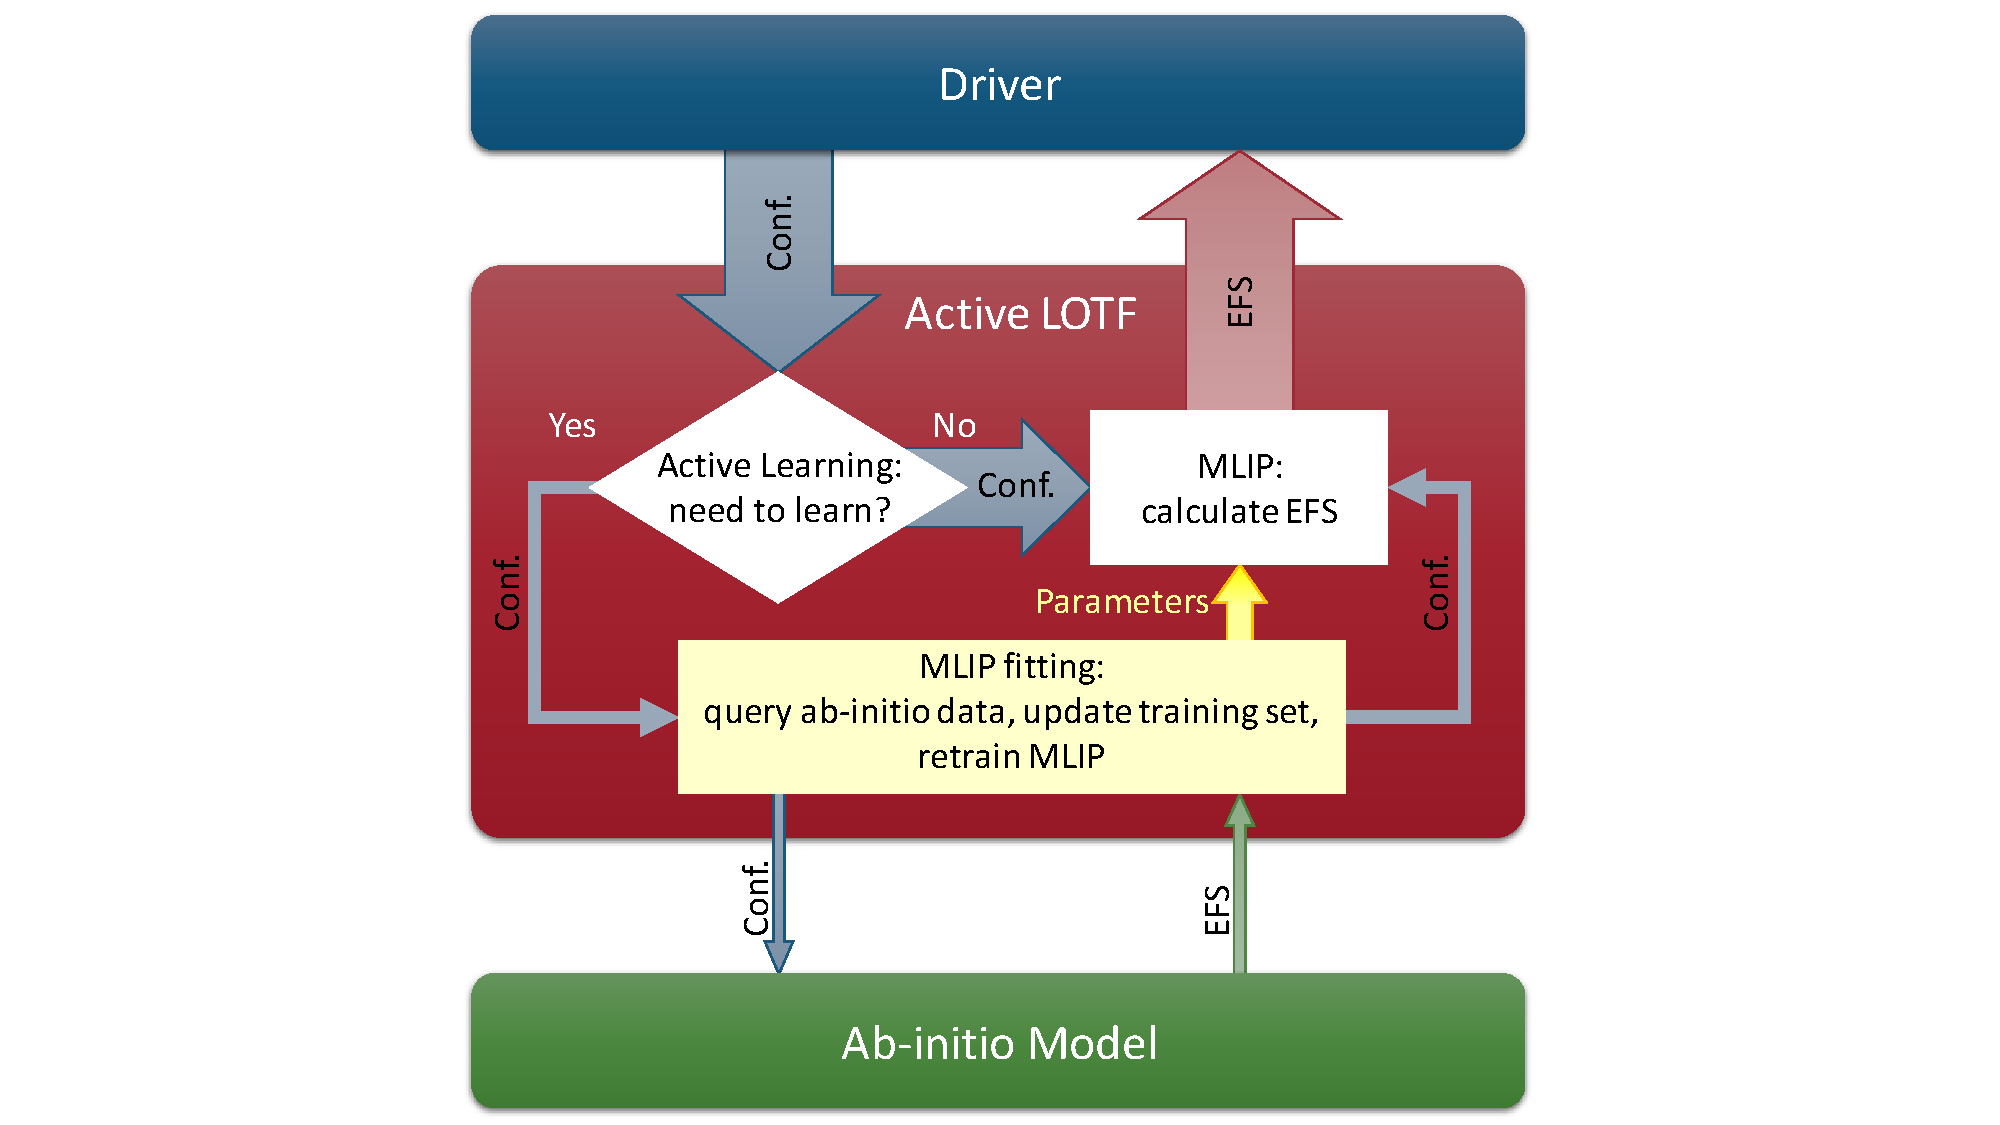
\includegraphics[width=4.0in]{figs/LOTF.pdf}
	\caption{Workflow in actively learning a potential on the fly.
		In the course of iterations an AL potential receives from MD a configuration and estimates the reliability of EFS calculation.
		If it detects sufficient extrapolation when calculating EFS, MLIP queries ab initio EFS, add this configuration to the training set, and retrains the potential.
		Then it calculates the EFS and passes it to the driver.
	}
	\label{fig:LOTF}
\end{figure}

\section{MLIP concept} \label{sec:concept}

MLIP, roughly speaking, provides tools for fitting potentials and using them in atomistic simulations.
MLIP, thus, can be used:
\begin{itemize}
\item
as a stand-alone package \texttt{mlp}, allowing for fitting the potentials and doing some simple atomistic simulations (see Section \ref{sec:install:mlp} for installation), and

\item as a plugin for external molecular modeling codes, like LAMMPS --- refer to the \texttt{INSTALL.md} file.
\end{itemize}

\begin{figure}
\begin{center}
\hfill
\subfigure[fitting on a database\label{fig:diagrams:fit}]{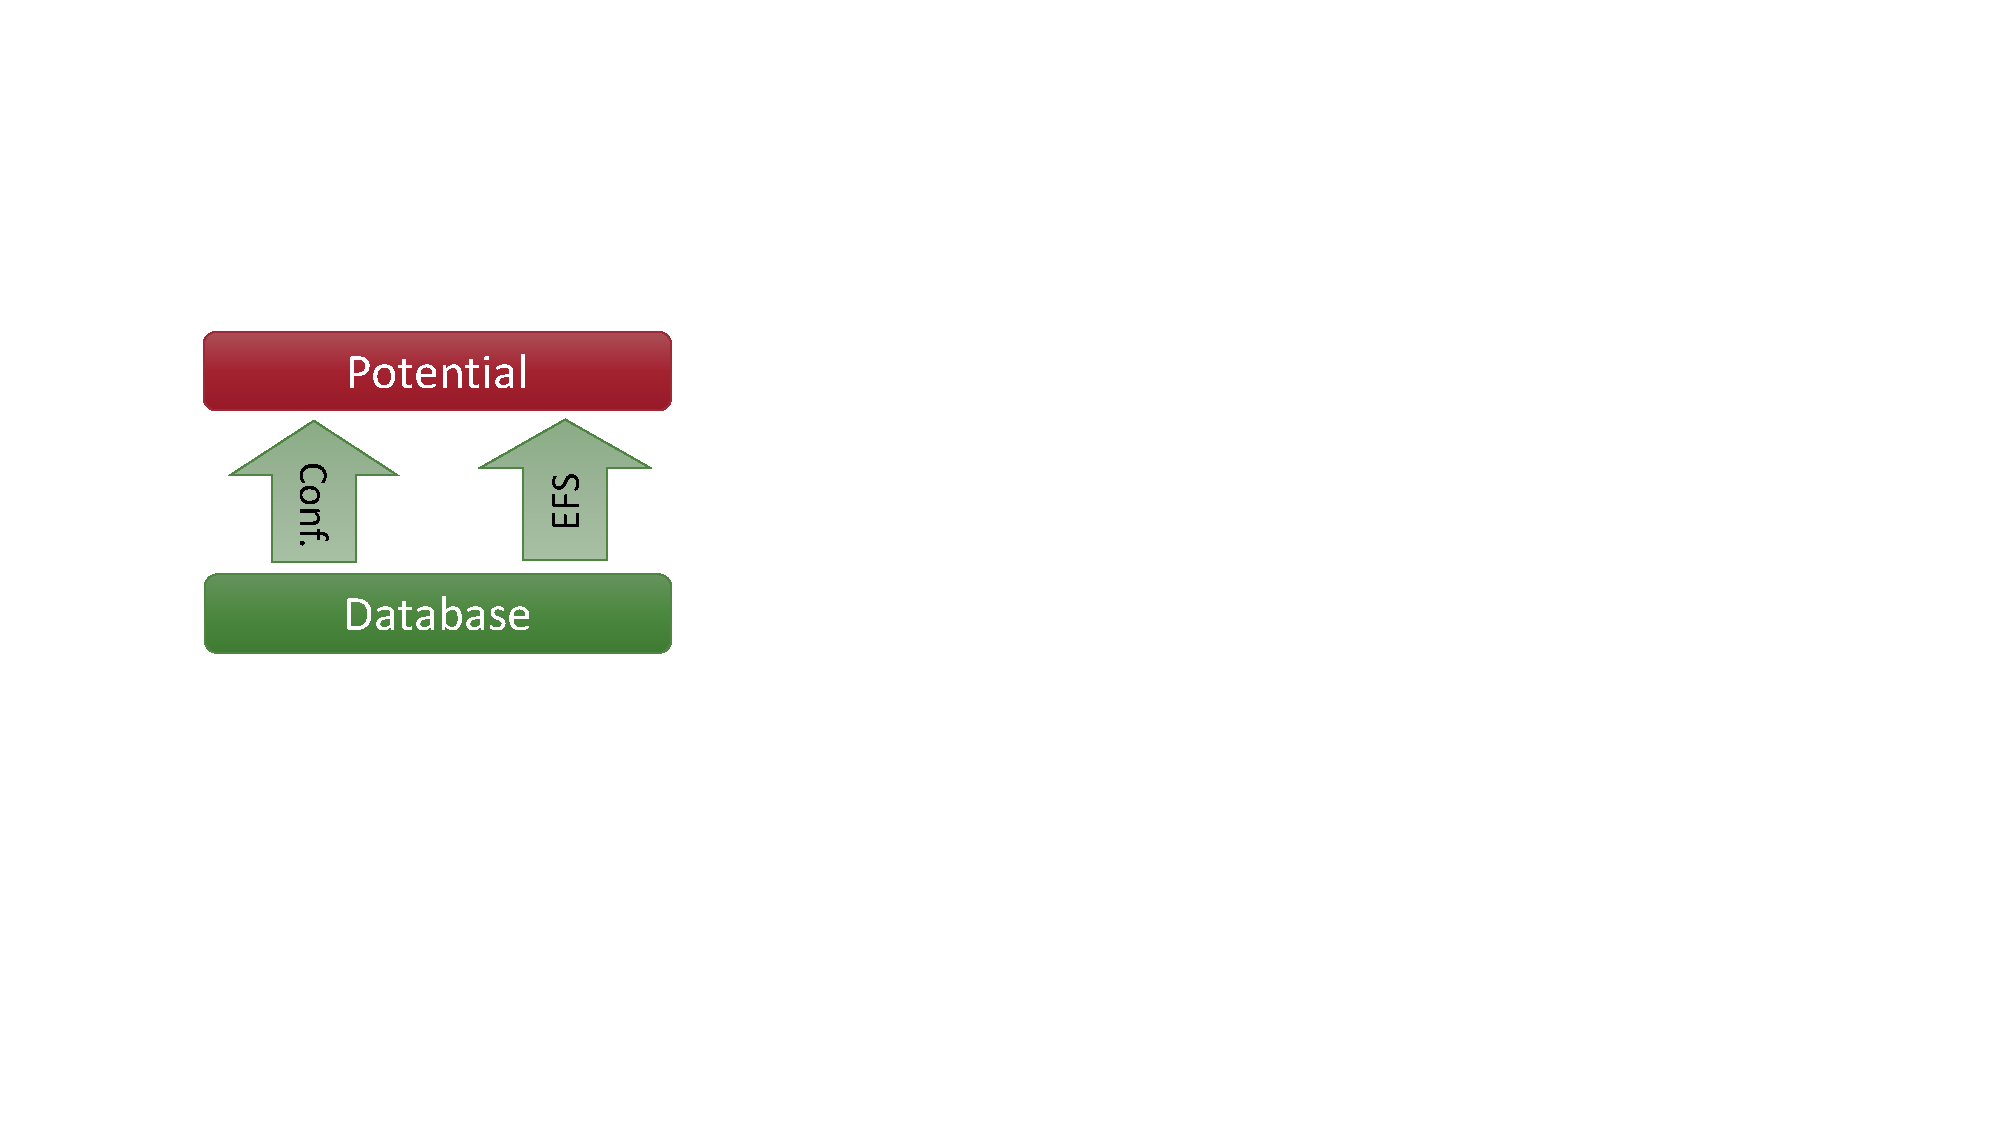
\includegraphics[page=1,scale=.5]{figs/diagrams.pdf}}
\hfill\hfill
\subfigure[simple atomisitic simulation\label{fig:diagrams:simple}]{\includegraphics[page=2,scale=.5]{figs/diagrams.pdf}}
\hfill\hfill
\subfigure[a learning-on-the-fly simulation\label{fig:diagrams:lotf}]{\includegraphics[page=3,scale=.5]{figs/diagrams.pdf}}
\hfill$\mathstrut$
\end{center}
\caption{Diagrams showing different ways of using MLIP: fitting and atomistic simulation.}
\label{fig:diagrams}
\end{figure}

The following is the typical use cases of MLIP:
\begin{itemize}
\item[(a)]
Fitting a potential on a configuration database (see Figure \ref{fig:diagrams:fit}).
This is achieved through \texttt{mlp train}.
The fitting errors (and validation errors) can be computed using \texttt{mlp calc-errors}.

\item[(b)]
A simple atomistic simulation with a trained potential (see Figure \ref{fig:diagrams:simple}).
Typically, this is done through LAMMPS.

\item[(c)]
A active learning type of simulation (see Figure \ref{fig:diagrams:lotf}).
This can be done both, through LAMMPS and \texttt{mlp run}.
\end{itemize}

%In fact, the scenario (c) encompasses all the other scenarios (at least in the serial version of MLIP).
%For example, (b) corresponds to (c) when Potential decides not to do any ab initio calculations, while (a) corresponds to (c) when Driver=``reading from a database'' and AIM=``preserve EFS as read from the database''.

More details are given in Section \ref{sec:aim}.

\section{Installation} \label{sec:install}

MLIP can use either a built-in BLAS or Intel MKL, or OpenBLAS (\url{http://www.openblas.net}) as a static library and is distributed as a part of this package (namely, OpenBLAS v.0.2.19 in the \texttt{blas/} folder). Use the \texttt{./configure} script to create a configuration.
Refer to the \texttt{INSTALL.md} file for more details.

\section{Usage examples} \label{Using}

The examples demonstrate the most frequently used routines.
All examples are available in \texttt{MLIP/test/examples/}.
Each example contain the launching script \texttt{test.sh}, the input files and the expected output in the \texttt{sample\_out} folder.
The output (normally) is written to the \texttt{out/} folder.

\section{MLIP file formats}

\subsection{CFG file}\label{cfg-file}

MLIP supports two internal formats for storing configurations in database files, typically having the ``\texttt{.cfg}'' extension: textual and binary.
We recommend using the binary format when the speed of input/output operations is critical.
The textual format, in contrast, is useful when configurations are prepared manually or converted from an unsupported format.

The example of configuration in the textual file format is bellow:

{\small
	\begin{verbatim}
	BEGIN_CFG
	 Size
	     12
	 Supercell
	        5.804540      0.000000      0.000000
	       -0.000052      4.304488      0.000000
	 AtomData: id type  cartes_x  cartes_y  cartes_z        fx        fy        fz
	            1    0  -0.06668   1.48178   2.12328   0.00116   0.00035   0.00023
	            2    1   1.23010   2.65535   1.49390  -0.00259  -0.00072   0.00170
	            3    0  -0.54459   4.36682   3.13176   0.00168   0.00059   0.00035
	            4    0   3.12308   2.65537   1.51976  -0.00075   0.00044  -0.00077
	            5    0   4.41954   1.48201   0.89064   0.00001  -0.00156  -0.00136
	            6    1   3.58878   3.89084   2.64425   0.00008   0.00077  -0.00044
	            7    0   3.44883   4.27728   0.83155   0.00105   0.00136   0.00081
	            8    0   0.46582   2.80689   3.10745  -0.00320  -0.00174  -0.00034
	            9    0   0.76409   3.89093   0.36959  -0.00025  -0.00035  -0.00032
	           10    1   3.30134   2.21479   3.25088   0.00283  -0.00171   0.00059
	           11    0   0.90387   4.27708   2.18219   0.00016   0.00292  -0.00053
	           12    0   2.29143   4.95920   3.27520  -0.00019  -0.00036   0.00006
	 Energy
	        -76.697992341920
	 Stress:  xx          yy          zz          yz          xz          xy
	    -0.00121     0.00075     0.00233     0.00191     0.00246    -0.00156
	 Feature    EFS_by    VASP
	 Feature    from      relaxation_driver
	 Feature    min_dist  1.734226
	 Feature    type_0    B
	 Feature    type_1    Al
	 Feature    comment	  
	 Feature    comment	   ((`'-"""-'`))
	 Feature    comment	    )  -   -  (
	 Feature    comment	   /   o _ o   \
	 Feature    comment	   \   ( 0 )   /
	 Feature    comment	    '-.._^_..-' 
	END_CFG
	\end{verbatim}
}

The description of each configuration in the database starts with \texttt{BEGIN\_CFG} and ends with \texttt{END\_CFG}. No symbols except whitespace (which is space, tab, and the newline characters '\textbackslash n' and '\textbackslash r') are allowed between configurations.
After \texttt{BEGIN\_CFG} several compulsory and optional fields follow. Bellow is the list of recognizable fields. 
\begin{enumerate}
	\item \texttt{Size} (compulsory field) is followed by one integer number, the number of atoms in the configuration.
	\texttt{Size} should appear before ``\texttt{AtomData:}''.
	
	\item \texttt{Supercell} (optional field) is followed by 3, 6, or 9 numbers, the 3 coordinates of the first lattice vector, then (optionally) 3 coordinates of the second lattice vector, and (optionally) 3 coordinates of the third lattice vector. 
	If \texttt{Supercell} is missing then no lattice vectors are given (this is a open-shell molecule).
	
	\item ``\texttt{AtomData:}'' (compulsory field) contains the per-atom data (atomic coordinates, forces, atom types, etc.). 		\texttt{AtomData:} is followed by one or more field names (on the same line):
	\begin{enumerate}
		\item \texttt{id} (optional field) means the ordinal number of atom in the configuration (1, 2, ...). If \texttt{id}'s are given, but are different from 1, 2, 3 in exactly in this order, it is an error.
		\item \texttt{type} (optional field) are the element types (0, 1, \ldots); if they are empty then all atoms are considered as of $0$ type and this is a single-component configuration.
		\item \texttt{cartes\_x}, \texttt{cartes\_y}, \texttt{cartes\_z} (all three are compulsory fields) means the Cartesian coordinates (measured in \AA).
		There is an alternative option to provide the configuration with direct (fractional) coordinates. In this case \texttt{direct\_...} caption should be specified instead of \texttt{cartes\_...}.
		\item \texttt{fx}, \texttt{fy}, \texttt{fz} (optional fields, but all three are required if present), are the force components in Cartesian coordinates (measured in eV/\AA).
		\item \texttt{site\_en} (optional field) is the site energy (in a rare occasion it is defined). 
		\item \texttt{charge} (optional field) may be used for storing of atomic partial charges.
	\end{enumerate}

	\item \texttt{Energy} (optional field) is followed by one number (measured in eV). 
	
	\item ``\texttt{Stress:}'' (optional field) must be immediately (on the same line) followed by the following 6 (not more and not less) field names (in any order), \texttt{xx}, \texttt{yy}, \texttt{zz}, \texttt{yz}, \texttt{xz}, and \texttt{xy}.
	On the next line are the 6 numbers, corresponding to those stresses.
	These are virial stresses multiplied by the cell volume (measured in eV).
	Positive stresses correspond to over-stretched configurations (in other words, ``stress = $-$force on the supercell'')
	
	\item ``\texttt{Feature}'' (optional fields, multiple entries are allowed) is/are additional (textual) attributes of a configuration (such as what chemical elements corresponds to the atom indexes, what generated it, what computed its energy, whether it is an ideal crystal or has a defect, etc.). Each ``Feature'' has a name (one word without whitespace) and value (a string separated from the name by a space or a tab character). A configuration may contain several features. 
	If two lines with the same name appear, the newline (`\texttt{\textbackslash n}') character and the second line are appended to the first line; similarly for the third line, etc.
	The features do not have universal meanings, they are used by different tools.
\end{enumerate}




\subsection{MTP file}\label{sup:mlip:mtp}

MTP file encodes a certain potential allowing for calculation energy, forces, and stresses of a configuration.

The objects, needed to calculate MTP basis functions (namlely, the parts of moment tensor descriptors), and MTP parameters are stored in \verb|.mtp| files. Here we describe the \verb|.mtp| file with the MTP of the level 8 before and after training. The example of empty MTP (before training) is shown below.
\begin{verbatim}
MTP
version = 1.1.0
potential_name = MTP1m
species_count = 1
potential_tag = 
radial_basis_type = RBChebyshev
min_dist = 2.25
max_dist = 6.2
radial_basis_size = 8
radial_funcs_count = 2
alpha_moments_count = 18
alpha_index_basic_count = 11
alpha_index_basic = {{0, 0, 0, 0}, {0, 1, 0, 0}, {0, 0, 1, 0},
{0, 0, 0, 1}, {0, 2, 0, 0}, {0, 1, 1, 0}, {0, 1, 0, 1},
{0, 0, 2, 0}, {0, 0, 1, 1}, {0, 0, 0, 2}, {1, 0, 0, 0}}
alpha_index_times_count = 14
alpha_index_times = {{0, 0, 1, 11}, {1, 1, 1, 12}, {2, 2, 1, 12},
{3, 3, 1, 12}, {4, 4, 1, 13}, {5, 5, 2, 13}, {6, 6, 2, 13},
{7, 7, 1, 13}, {8, 8, 2, 13}, {9, 9, 1, 13}, {0, 10, 1, 14},
{0, 11, 1, 15}, {0, 12, 1, 16}, {0, 15, 1, 17}}
alpha_scalar_moments = 9
alpha_moment_mapping = {0, 10, 11, 12, 13, 14, 15, 16, 17}
\end{verbatim}
There are two groups of objects in the file: the objects that could be changed by a user, and the unchangeable objects related to the level and particular functional form of the MTP.
%\newpage
First we describe the hyperparameters that could be adjusted by the user.
\begin{description}[style=nextline,leftmargin=\widthof{\ttfamily radial\_basis\_sizeX|},font=\normalfont\ttfamily]
	\item[species\_count] is the number of components (atomic types) in the system investigated;
	\item[radial\_basis\_type] is the type of radial basis used (the most frequently used radial basis is the Chebyshev basis);
	\item[min\_dist] is the minimal distance between atoms in the training set (in angstroms);
	\item[max\_dist] is the cut-off radius (in angstroms);
	\item[radial\_basis\_size] is the size of radial basis (the Chebyshev basis for this MTP).
\end{description}
The second group of the objects cannot be freely modified by a user. They are:
\begin{description}[style=nextline,leftmargin=\widthof{\ttfamily XXX|},font=\normalfont\ttfamily]
	\item[radial\_funcs\_count] is the maximum number of radial functions $f_{\mu}$ which is necessary to create all possible MTP basis functions for a specified MTP level (e.g., for the MTP of the level 8 it is necessary to consider two radial functions);
	\item[alpha\_moments\_count] is the total number of the objects, written in the MTP file, which are the parts of the moment tensor descriptors, yielding a scalar, and not greater than a specified level;
	\item[alpha\_index\_basic\_count] is the number of basic objects (i.e., the objects, that were not multiplied by the other objects);
	\item[alpha\_index\_basic] are the basic objects, including the indices of radial functions (the first indices, could be equal to 0 or 1, because only two radial functions needed to construct all MTP basis functions), and the powers of $x_{ij}$, $y_{ij}$, $z_{ij}$ (the second, the third, and the fourth indices, correspondingly);
	\item[alpha\_index\_times\_count] is the number of complex objects (i.e., the ones, obtained by pairwise multiplying of objects);
	\item[alpha\_index\_times] are the pairwise multiplied complex objects, including the indices of two objects multiplied (the first and the second indices), the number of such the objects (i.e., the factor before multiplication, the third indices), and the number of complex object (the fourth indices, we emphasize, that the basic objects enumerated automatically, one ny one, we do not keep their indices); \item[alpha\_scalar\_moments] is the number of the MTP basis functions; and, finally,
	\item[alpha\_moment\_mapping] are the indices of basis and complex objects, forming the MTP basis functions.
\end{description}
For example, for the current MTP of the level 8 there are 9 MTP basis function \eqref{eq:MTPbasisLevel8}, therefore, $\verb|alpha_scalar_moments| = 9$ and we need the objects with the indices \verb|alpha_moment_mapping| to form the MTP basis functions \eqref{eq:MTPbasisLevel8}.\\

\noindent After the fitting of the MTP, the parameters of fitting added in \verb|.mtp| file: the strings with $\verb|radial_basis_size| \times \verb|radial_funcs_count|$ radial coefficients
\begin{verbatim}
radial_coeffs
0-0
{-4.243215058993401e-01, -7.013766150563229e-01, ... }
{8.483313776829586e-02, -2.944665241055562e-02, ... }
\end{verbatim}
the string with energies of individual atoms, one per atomic type,
\begin{verbatim}
species_coeffs = {-4.699403701006758e+00}
\end{verbatim}
and the strings with 9 linear coefficients
\begin{verbatim}
moment_coeffs = {1.0466030834e+00, 6.5878384919e-01, ...}
\end{verbatim}

\subsection{ALS file}\label{sup:mlip:als}

A \verb|.als|-file stores the selection state data, including the MTP, and the active set. It has a mixed text/binary structure and is organized as follows. First it contain the fitted MTP. Next the selection weights are specified. After that a binary part follows. It contain a binary representation of active selection matrix $\mathsf A$ and $\mathsf A^{-1}$. Actually these matrices can be recalculated from the active set that is stored later, however this data helps to prevent the change of the selection state after loading due to rounding errors.
Next, a block with the configurations corresponding to the matrix rows are stored.
At the end of the \verb|.als|-file the active set (in \verb|.cfg|-format with full floating-point precision) is writen. 

\subsection{mlp binary file}\label{sup:mlip:mlp}

The \verb|mlp| binary file allows to run various MLIP code commands. To list the most frequently used MLIP commands, execute \verb|mlp list|. To provide a description of some command, execute \verb|mlp help [command]|. A typical template of the rest commands available is 
\begin{verbatim}
mlp [command] [input/output files] [options]
\end{verbatim}
The main MLIP commands (or, their examples) and description are shown below.
\begin{description}[style=nextline,leftmargin=\widthof{\ttfamily XXX|},font=\normalfont\ttfamily]
	\item[mlp relax mlip.ini --cfg-filename=to\_relax.cfg --save-relaxed=relaxed.cfg] Relaxation of configurations in the file \verb|to_relax.cfg| in accordance with the settings in \verb|mlip.ini|, writing the result in the file \verb|relaxed.cfg|.
	\item[mlp convert-cfg <input-filename> <output-filename> --options ]
	Converting of an atomic configuration from a format of \verb|input-filename| to a configuration in a format of \verb|output-filename|. All the formats, except for internal MLIP \verb|.cfg|, should be specified, e.g.
	\begin{verbatim}
	mlp convert-cfg input.cfg POSCAR --output-format=vasp-poscar
	\end{verbatim}
	\item[mlp train init.mtp train.cfg --trained-pot-name=pot.mtp ]
	Training of MTP in the \verb|init.mtp| file on the dataset in \verb|train.cfg| file. The option \verb|trained-pot-name| indicates that the potential trained is written in the \verb|pot.mtp| file.
	\item[mlp calc-errors pot.mtp db.cfg ]
	Calculation of the prediction errors by the \verb|pot.mtp| potential on the database in \verb|db.cfg|.
	\item[mlp calc-efs pot.mtp in.cfg out.cfg ]
	Calculation of energies, forces, and stresses for the configurations in \verb|in.cfg| with the \verb|pot.mtp| potential, writing the result in \verb|out.cfg|.
	\item[mlp calc-grade pot.mtp train.cfg in.cfg out.cfg --als-filename=state.als ]
	Creation of the \verb|state.als| file with maxvol state for the potential \verb|pot.mtp| fitted on the database written in \verb|train.cfg|. Calculation grades of configurations in the \verb|in.cfg| file, writing the configurations with grades calculated in the \verb|out.cfg| file.
	
	\item[mlp select-add pot.mtp train.cfg preselected.cfg add\_to\_train.cfg ]
	Maxvol selection of non-pereative configurations from \verb|preselected.cfg|, writing of the selected configurations in the \verb|add_to_train.cfg| file for further adding of these configurations to the \verb|train.cfg| file.
	
\end{description} 

\subsection{MLIP settings}\label{sec:mlip:ini}

Settings file, typically named as \verb|mlip.ini|, is required when MLIP is used from LAMMPS as \verb|pair_style|, namely
\begin{verbatim}
pair_style  mlip mlip.ini
pair_coeff  * *
\end{verbatim}
The same file can be used with the \verb|mlp relax| command to specify what MTP file to use and whether or how active learning should be used.
It contains the instructions and settings for MLIP determining the operational regime.
An example of a simple \verb|mlip.ini| is below:
\begin{verbatim}
mtp-filename          pot.mtp
select                FALSE   # turned off for a large-scale MD run
\end{verbatim}
More examples of settings file can be found in examples provided with the MLIP package.

The \verb|mlip.ini| file is organized according the following rules.
\begin{itemize}
	\item Each setting is given in a separate line and have the form 
	\begin{verbatim}
	identifier    value
	\end{verbatim}
	where \texttt{identifier} is the string without whitespace and \texttt{value} is another string without whitespace (a string can be a number). They must be separated by any number of spaces or tab symbols.
	Whitespace before \texttt{identifier} as well as any symbols after \texttt{value} are allowed but ignored by the parser. 
	
	\item Other than identifiers and values, the lines of the settings file can contain comments. Comments begin with ``\texttt{\#}'' and all the foregoing symbols are ignored in this line. 
	
	\item The order of lines is not important; therefore the lines can be grouped for the user's convenience.
	
	\item If a parameter is not present (or commented out), its default value is used. 
	
	\item If a setting is not supported then it is ignored (without a warning).
\end{itemize}

The recognizable identifiers and their meaning are listed below.
\begin{description}[style=nextline,leftmargin=\widthof{\ttfamily XXX|},font=\normalfont\ttfamily]
	\item[mtp-filename   <filename>] File name with MTP to be loaded.
	\item[write-cfgs   <filename>] if this setting is present then the processed configurations will be written to the specified file, may be useful for debug.
	\item[write-cfgs:skip   <number>] skip this many configurations before writing a processed configuration.
	\item[select   <TRUE/FALSE>] activates or deactivates calculation of extrapolation grades and optionally writing configurations with high extrapolation grades. Can be combined with (or run independent from) energy, forces and stresses calculation. If \texttt{false} value is specified the following settings will be ignored.
	\item[select:threshold   <real number>]  corresponds to $\gamma_{\rm select}$ mentioned in Section \ref{sec:AL}. If the extrapolation grade exceeds this value configuration will be saved to a file with extrapolative configurations met.    
	\item[select:threshold-break   <real number>]  corresponds to $\gamma_{\rm break}$ mentioned in Section \ref{sec:AL}. If the extrapolation grade exceeds this value the program execution will be interrupted, that can be used for prevention of instability of the simulation.    
	\item[select:load-state   <filename>] a file for loading the selection state.
	\item[select:log   <filename>/stdout/stderr] a file (or standard output stream) for writing a log of configuration selection with the extrapolation grades of treated configurations.
\end{description}

\section{Feedback}
We will later, once the status of this manual changes, provide an email for user feedback.
%If you run into problems with MLIP or if you have a some related questions, please contact Alexander Shapeev (\texttt{mlip.soft@gmail.com}).

\bibliography{manual}

\end{document}
